\subsection{Resultado - Exercício 4}

Os passos são:
\begin{itemize}[leftmargin=3.5em, itemsep=-.5mm, topsep=0.5mm]
    \item Calcular a séria para a função $f(x) = \frac{1}{1 - x}$
    \item Aplicar $t^2$ no resultado
    \item Comparar e aplicar com a função $f(x) = arctan(x)$
    \item Problemas com a série
    \item Melhoramentos para redução das diferenças
    \item Apresentação dos testes solicitados
    \item Apresentar o código Python
\end{itemize}

\newpage

\subsubsection{Calcular a séria para a função $f(x) = \frac{1}{1 - x}$}
\begin{figure}[H]
    \centering
    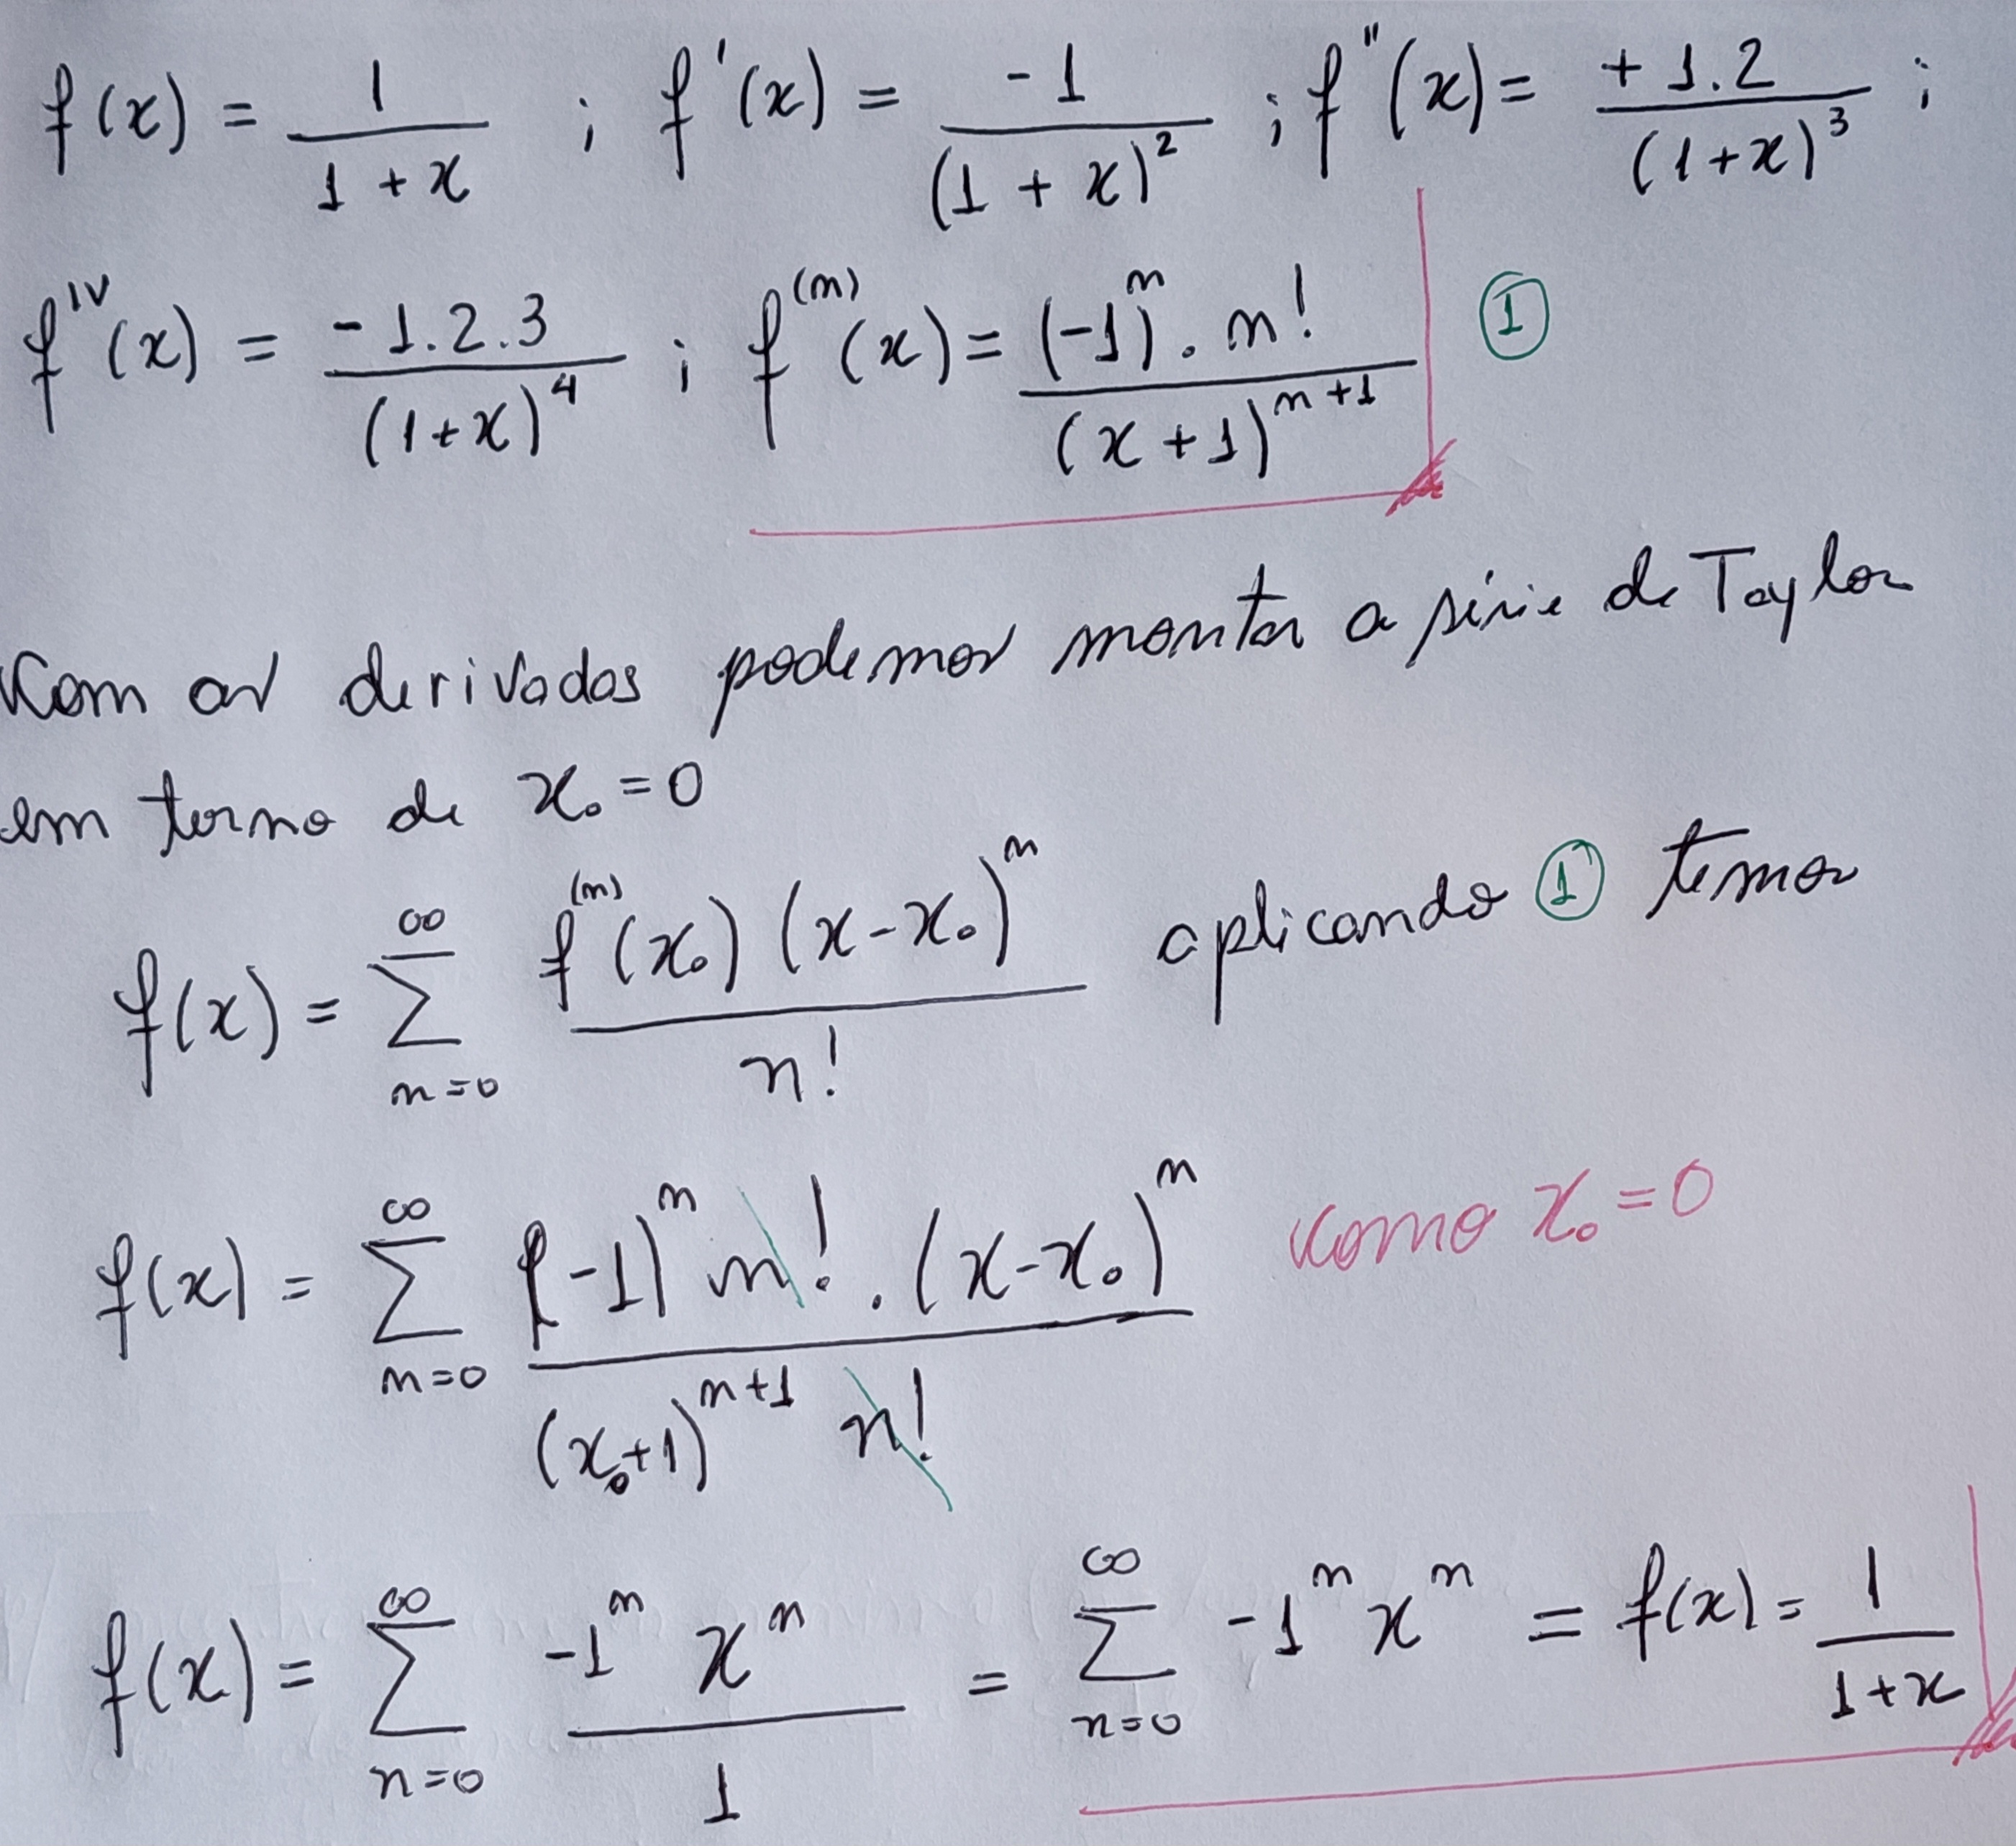
\includegraphics[width=.7\textwidth]{imagens/exercicio4_parte1}
    \caption{Calculando a série de Taylor de $f(x) = \frac{1}{1 - x}$}
    \label{fig:exe4_parte1}
\end{figure}

\subsubsection{Aplicar $t^2$ no resultado}

Ao aplicar $t^2$ em $f(x)$ definida pela série $f(x) = \sum_{n=0}^{\infty} (-1)^n \cdot x^n $ ou escrita na forma:

$f(x) = 1 - x + x^2 - x^3 + x^4 - x^5 \mathellipsis $ \\
Agora teremos como resultado

\begin{figure}[H]
    \centering
    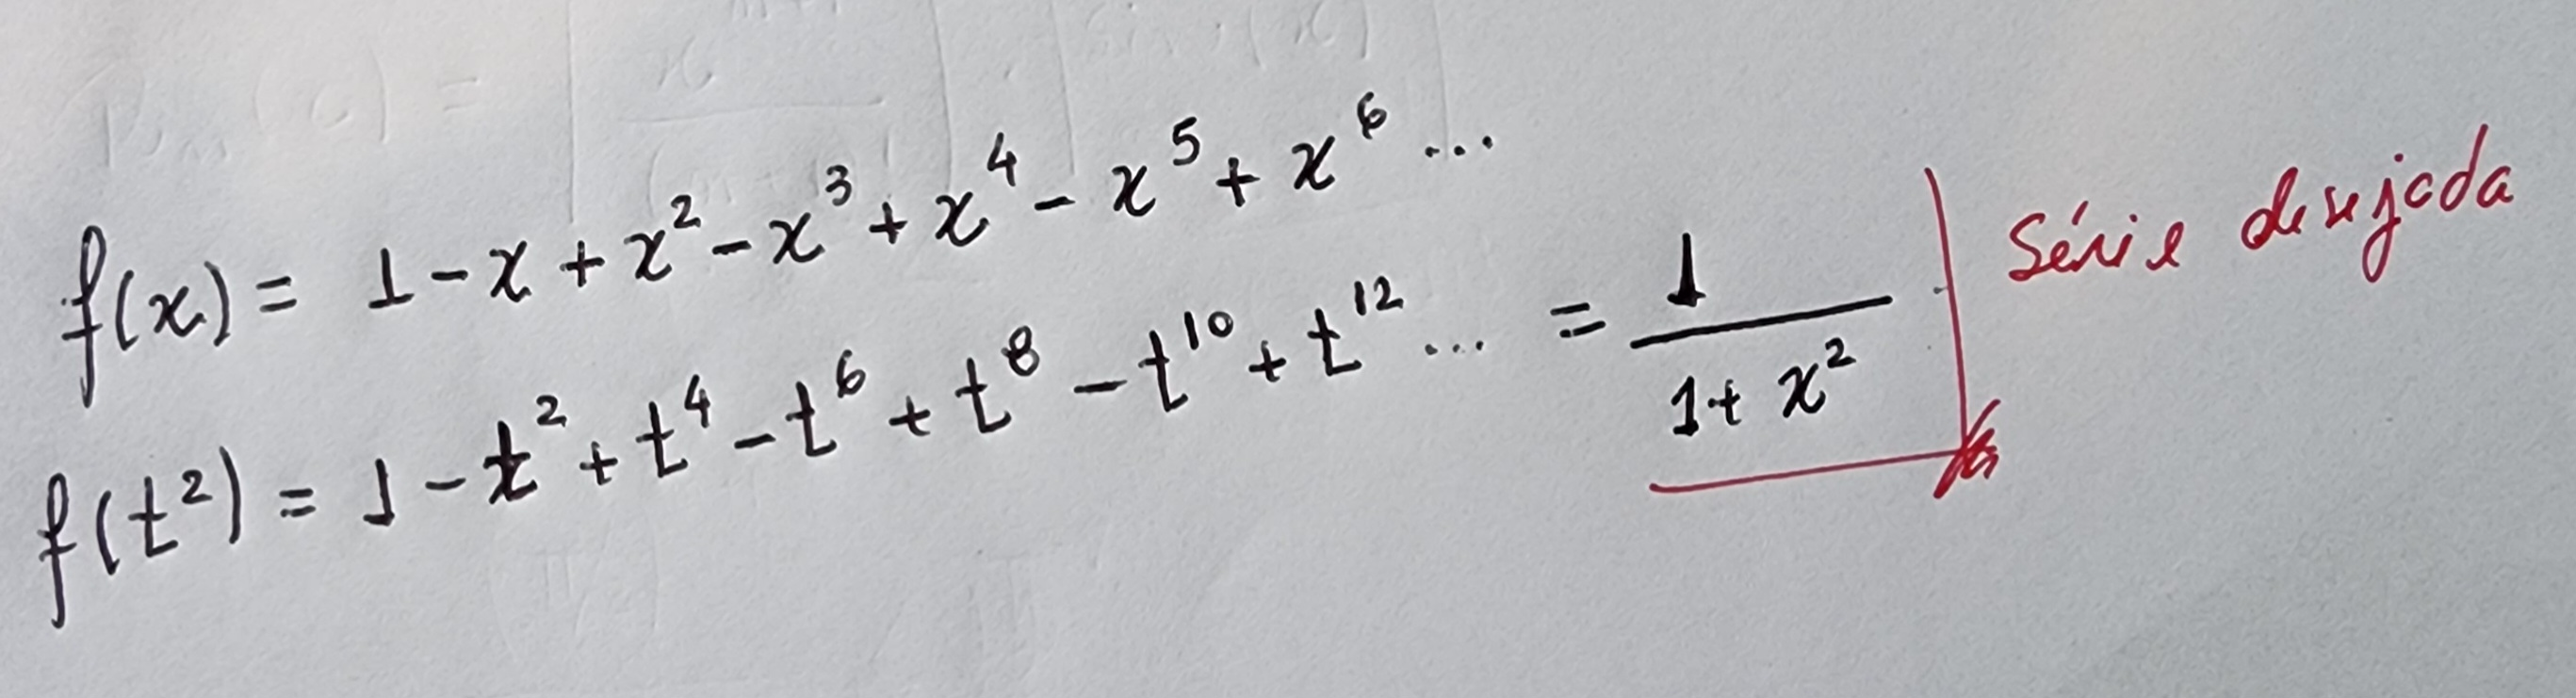
\includegraphics[width=1.0\textwidth]{imagens/exercicio4_parte2}
    \caption{Calculando a série de Taylor desejada $f(x) = \frac{1}{1 - x^2}$}
    \label{fig:exe4_parte2}
\end{figure}

A Figura~\ref{fig:exe4_parte2} mostra que o resultado da expansão usando a série de Taylor para $f(t) = \frac{1}{1 + t^2}$ é

$f(t) = \sum_{n=0}^{\infty} (-1)^n \cdot t^{2 \cdot n}$

\subsubsection{Comparar e aplicar com a função $f(x) = arctan(x)$}

\begin{figure}[H]
    \centering
    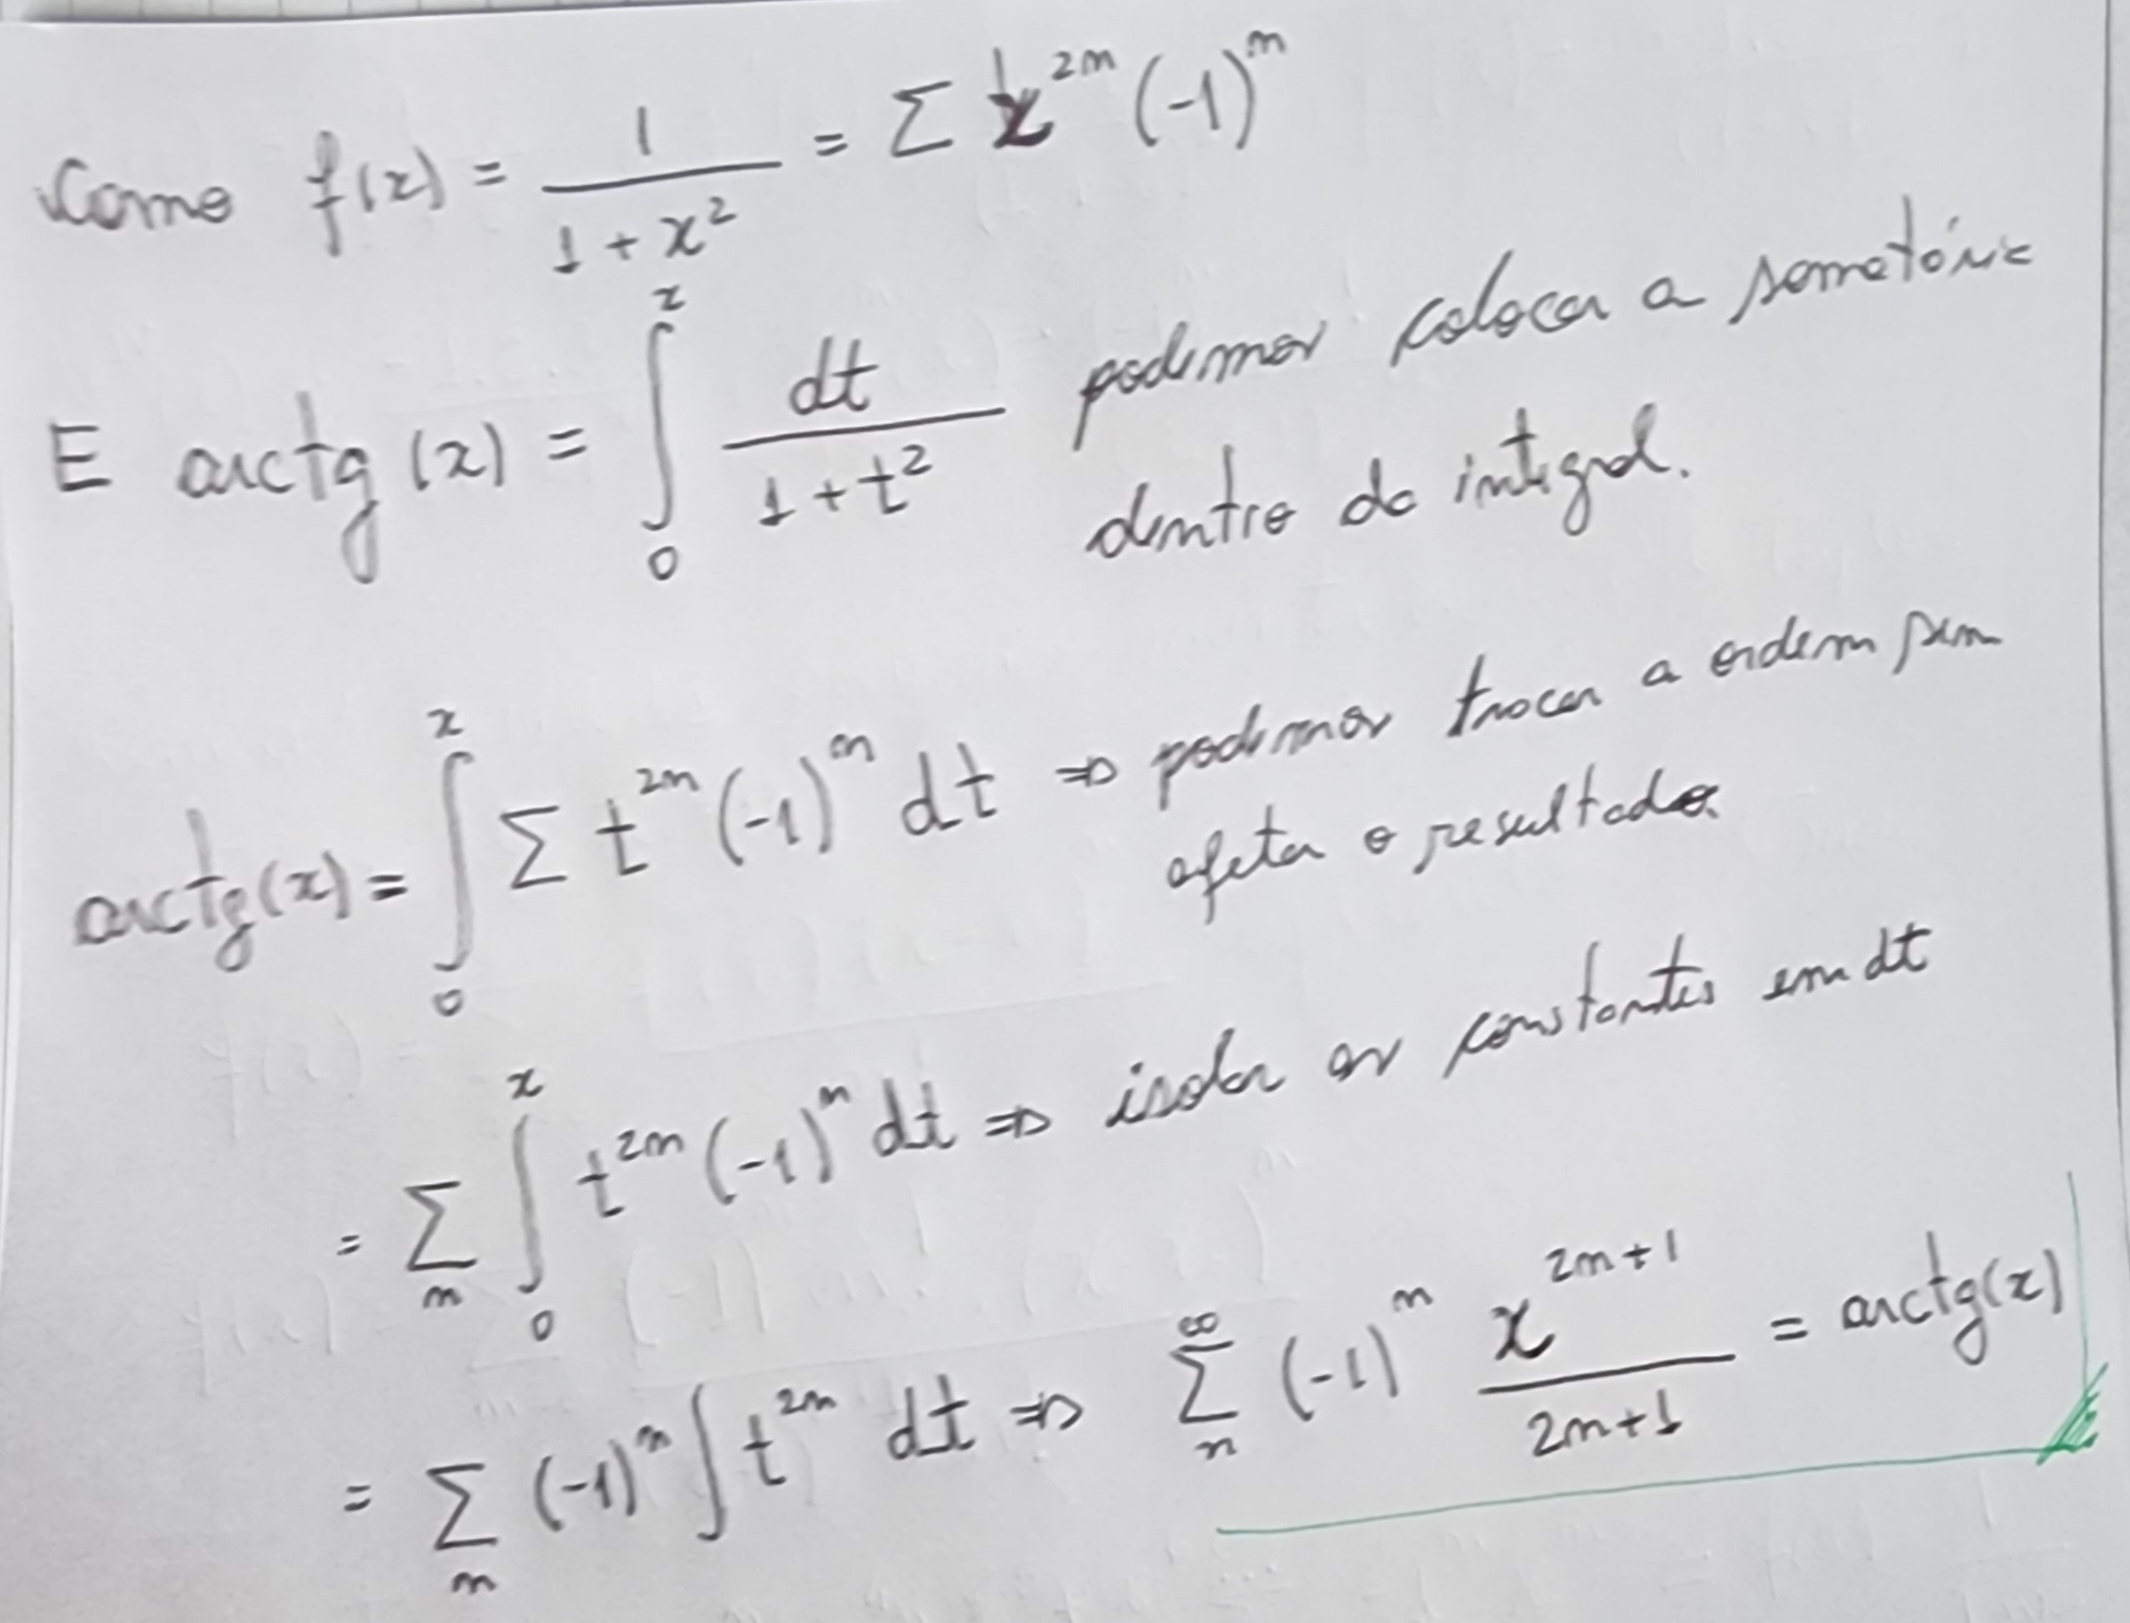
\includegraphics[width=.7\textwidth]{imagens/exercicio4_parte3}
    \caption{Calculando a série de Taylor para $f(x) = arctan(x)$}
    \label{fig:exe4_parte3}
\end{figure}

Assim temos que $f(x) = arctan(x) = x + \frac{-x^3}{3} + \frac{x^5}{5} + \mathellipsis + \frac{(-1)^n \cdot x^{2 \cdot n + 1}}{2 \cdot n + 1} $

\subsubsection{Problemas com a série}

Foi implementado a série usando o algoritmo de Hormer com sucesso, no entando, para valores acima de um $(1.0)$ a série diverge.
Isso causa um erros consideráveis. Parar evitar esse problema utilizamos relações trigonométricas do site \cite{site-geek} para manter o valor de x menor que 1.

Isso foi colocado no código na função \texttt{calcula\_f\_x\_taylor\_com\_horner\_ajustado}. Está sendo utilizado algumas características do \texttt{arctan} para ficarmos entre $0.$ e $1.$ além das simetrias de uma função impar.

\subsubsection{Melhoramentos para redução das diferenças}
\label{sec:melhoramentos-serie-arctan}
Foi usado a caractéricas que $arctan(-x) = -arctan(x)$. Essa característica mantém os valores de $x$ sempre no domínio positivo.\\
Outra característica foi usada para manter o domínio de x entre 0 e 1 que foi:
\begin{itemize}
    \item[] $\arctan\left(\frac{1}{x}\right) = \frac{\pi}{2} - \arctan(x) = \mathrm{arccot}(x), \quad \text{se } x > 0$
\end{itemize}

O resultado final dos ajustes está na Tabela~\ref{tab:exercicio_4_resultados} e são muito significativos.\\

Executando o programa com 60 mil valores de $-300$ a $+299.99$ temos:

\begin{table}[h!]
    \centering
    \caption{Quadro comparativo com valores entre $-300$ e $299.99$ com séria de $arctan(x)$ usando e não usando ajuste considerado em \cite{site-geek}}
    \label{tab:exercicio_4_critica_1}
    \begin{tabular}{|c|c|c|c|c|}
        \hline
        \textbf{Tipo} & \textbf{Quantidade Total} & \textbf{Erros $>1\%$} & \textbf{Erros $<1\%$} & \textbf{Intervalo com erro $>1 \%$} \\
        \hline
        Com Ajuste & 60.000 & 11 & 59.989 & [0.95 , 1.05] \\
        Sem Ajuste & 60.000 & 29906 & 30095 & [0.95 , 300.] \\
        \hline
    \end{tabular}
\end{table}

Analisando os intervalos de valores com erro segundo Tabela~\ref{tab:exercicio_4_critica_1}, os 11 valores com erro maior que $1 \%$ ficam entre $0.95$ e $1.05$.
Ao contrário do que acontece quando não realizamos o ajuste. A quantidade, neste último caso, é praticamente $50 \%$ dos itens que testamos em quase todo o range tal que o módulo de $x$ é maior que $0.95$.\\
Assim, o ajuste foi muito eficiente e reduz substancialmente a quantidade de erros devido a convergência da série usada.

\subsubsection{Apresentação dos testes solicitados}
    
    \begin{table}[h!]
    \centering
    \caption{Testes do Exercicio 4}
    \label{tab:exercicio_4_resultados}
    \begin{tabular}{|c|c|c|c|c|c|}
    \toprule
    \textbf{$x$} & \textbf{$f(x)$ (NP)} & \textbf{$P_{10}(x)$  s/ ajuste} & \textbf{$P_{10}(x)$ c/ ajuste} & \textbf{Dif. sem ajuste} & \textbf{Dif. com ajuste}\\
    \midrule
    
    1.5708e+00 & 1.0039e+00 & -1.9211e+02 & 1.0039e+00& 1.9311e+02 & 2.6472e-06 \\
                          1.0472e+00 & 8.0845e-01 & 7.4565e-01 & 8.1833e-01& 6.2802e-02 & 9.8820e-03 \\
                          7.8540e-01 & 6.6577e-01 & 6.6558e-01 & 6.6558e-01& 1.9103e-04 & 1.9103e-04 \\
                          
    \bottomrule
    \end{tabular}
    \end{table}    
    

\subsubsection{Apresentar o código Python}
    \lstinputlisting[style=python]{scripts/exercicio4.py}
    Código para solução e testes do exercício 4.
